\documentclass{article}

\usepackage{amsmath}
\usepackage{amsthm}
\usepackage{graphicx}
\usepackage{hyperref}
\setlength{\parskip}{1em}

\begin{document}

    \title{EOPSY lab 4 report}
    \author{Michał Szopiński 300182}
    \date{June 13, 2021}
    \maketitle
    
    \section{Overview}
    
    The goal of this laboratory was to gain insight into memory management
	mechanisms is operating systems. For this purpose, a memory mapping
	simulator was used and its output was observed.
	
	\section{Theory}
	
	An operating system aims to distribute the resources available in a
	computer across many processes, so that each one of them may use the
	resources without conflict. In the case of memory, a technique known as
	virtual memory is used, in which contiguous regions of the address space
	visible to a process are mapped onto various parts of physical memory.
	
	Said regions are known as pages -- fixed-sized chunks of
	address space which correspond to different physical addresses. If a
	process tries to access a virtual page which has not yet been assigned
	a physical mapping, a page fault occurs. The OS resolves the page fault and
	finds a suitable mapping using various algorithms, including:
	
	\begin{enumerate}
        \item First in, first out -- the pages are reused based on a simple
		FIFO queue
        \item Least recently used -- the OS keeps track of when a page was last
		used and picks the one that hasn't been used for the longest time
    \end{enumerate}
	
	\section{Laboratory task}
	
	The task was to map the first 8 pages of virtual memory onto the first 8
	pages of physical memory, and then to attempt to access all 64 virtual
	pages.
    
	\begin{figure}[h]
		\begin{center}
			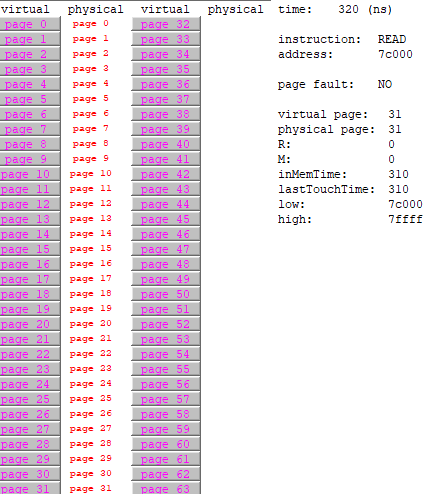
\includegraphics[width=0.4\linewidth]{screenshot1.png}
			\caption{The first 32 pages read without page fault.}
			\label{fig:topview}
		\end{center}
	\end{figure}
	\begin{figure}[h]
		\begin{center}
			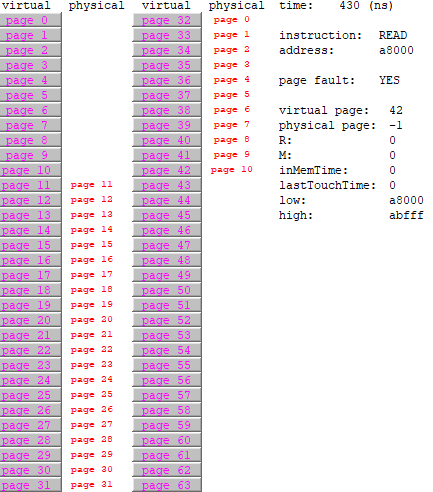
\includegraphics[width=0.4\linewidth]{screenshot2.png}
			\caption{Pages 32 onwards being remapped due to page fault.}
			\label{fig:topview}
		\end{center}
	\end{figure}
	\begin{figure}[h]
		\begin{center}
			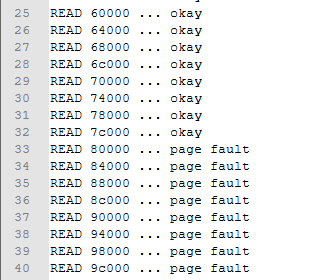
\includegraphics[width=0.5\linewidth]{screenshot3.png}
			\caption{The moment of the page fault captured in the trace file.}
			\label{fig:topview}
		\end{center}
	\end{figure}
	\begin{figure}[h]
		\begin{center}
			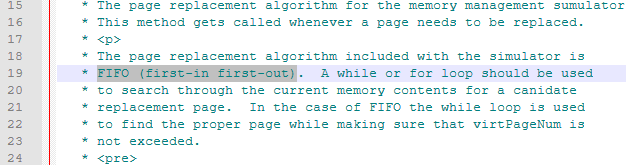
\includegraphics[width=1\linewidth]{screenshot4.png}
			\caption{The page replacement algorithm as described in the source.}
			\label{fig:topview}
		\end{center}
	\end{figure}
	
	\clearpage
	
	As evident from the screenshots, the first 8 pages of the virtual memory
	were successfully accessed without a page fault. Interestingly, so did the
	following 24. This is presumably due to a default mapping in the simulator.
	
	Starting from page 32, however, page faults started occuring. These were
	resolved by a page replacement algorithm. Analysis of the assigned pages
	reveals that the replacement algorithm is FIFO -- lower pages have priority
	over higher pages. This is confirmed by looking at the source code of the
	simulator.
	
\end{document}
